\section{引言}
大型语言模型（LLM）的快速发展催生了丰富的应用场景，包括交互式聊天机器人~\cite{zheng2023judging,chiang2023vicuna,openai2024gpt4}、代码助手~\cite{liu2024exploring,zhong2024can}以及智能体系统~\cite{talebirad2023multi,he2025llm,yu2024fincon}。现代服务系统必须在维持海量请求吞吐的同时，满足异构服务级目标（SLO）~\cite{tempo2025,patke2024queue,hongsola,chen2025slos,shen2025accelgen}，以支撑严格的性能预期。在这些指标中，首 Token 时间（TTFT）尤为关键，因为它既决定了交互式用户所感知到的响应性~\cite{wang2024revisiting,ethiraj2025toward}，也关系到智能体流水线中的严格超时约束~\cite{LiteLLM,langfuse,notdiamond}。TTFT 目标被违反时，往往会触发重复重试~\cite{Medium1,Medium2}，造成不必要的资源消耗~\cite{mooncake}与显著营收损失~\cite{ranganathan2025enhancing}。

\begin{figure}[t!]
    \centering
    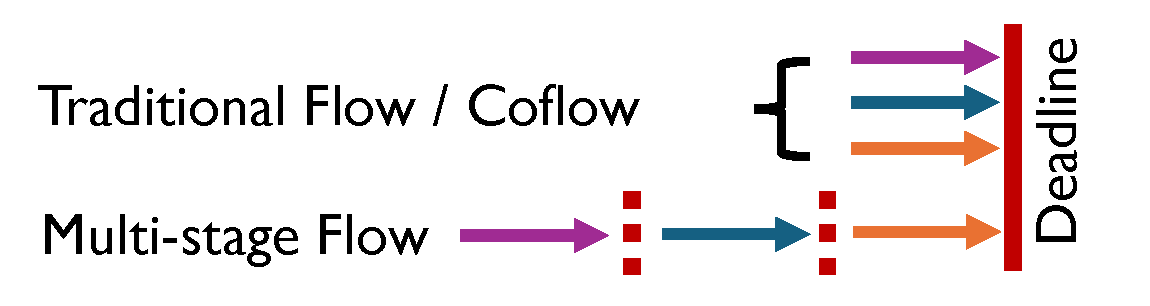
\includegraphics[width=0.9\linewidth]{figures/intro/multistageflow.pdf}
    \caption{多阶段流调度与以往“与阶段无关”调度方式差异示意图。}
    \vspace{-1.5em}
    \label{fig:intro:MFS}
\end{figure}


现代 LLM 服务系统通常采用带 KV-cache 复用的 Prefill--Decode 解耦架构~\cite{distserve,splitwise,strati2024d,hu2024inference,mooncakefast,hu2024memserve,cachedattention,cacheblend}，并利用多种并行方式~\cite{expertparallel,deepspeedMoE,deepseektech,comet}来提升效率。尽管这些设计前景可观，它们在 prefill 阶段仍然承受着显著的通信开销。具体而言，生成第一个 token 涉及\emph{多阶段}通信：(1) 远程检索可复用的 KV 块；(2) 为中间激活同步而进行的集合通信；(3) Prefill-to-Decode（P2D）传输。不同阶段的流经常会在共享网络上重叠并相互竞争，从而产生\emph{请求内争用}——同一请求内部不同通信阶段彼此干扰，以及\emph{请求间争用}——来自不同 batch 或不同 prefill 单元的通信竞争相同链路。这类争用会显著拉长 prefill TTFT 延迟，并提升系统范围内 SLO 违约的风险。

遗憾的是，现有工作在争用条件下无法满足端到端截止期限（见图~\ref{fig:intro:MFS}），主要原因在于它们以与阶段无关的方式处理流（即忽视阶段依赖）。传统流调度方案（如 Fair Sharing~\cite{dctcp,dcqcn}、SJF~\cite{pfabric,PDQ,pias,li2024flow}、EDF~\cite{D3,d2tcp,PDQ} 等）只针对单个流做决策，缺乏整体视角。即使是 coflow 方案~\cite{varys,Aalo,zhang2016coda,zhao2015rapier,agarwal2018sincronia,wan2025coflow}也存在不足：它们虽然能把数据并行流作为一个组来管理，却忽视了各阶段之间的内在依赖。因此，这些方案可能过度优先早期阶段通信，或让对时延敏感的下游阶段被饿死，最终损害 TTFT SLO 达成率。

基于此，我们提出一个问题：\emph{能否在 LLM 服务系统中以整体方式调度多阶段通信，从而最大化总体 TTFT SLO 达成率？}

在探索设计空间时，我们注意到已有一些工作分别针对孤立阶段进行优化，目标要么是集合通信~\cite{rajasekaran2024cassini,cao2024crux,xu2025autoccl,cao2025syccl,si2025collective}，要么是 KV-cache 传输~\cite{strati2024d,cachegen,chen2024kvdirect,mooncakefast}。然而，这些专用方案仍然不够。原因在于，它们常常追求彼此冲突的优化目标，若简单叠加，反而可能放大网络争用。

本文给出的答案是肯定的。我们提出 \sys{}，一种\emph{整体式}多阶段通信调度器，用于联合编排存在依赖关系的各通信阶段，以最大化 TTFT SLO 达成率。我们的关键洞见是：随着 prefill 执行推进，全局 TTFT 截止时间可以逐步转化为显式的流级截止时间。基于这一观察，\sys{} 在不确定环境下近似 Least-Laxity-First（LLF）策略，并通过反向多级队列（RMLQ）实现 \emph{延后并提升} 原则。通过依据有效松弛度的缩小动态提升任务优先级，\sys{} 能优先保障真正关键的阶段，同时避免 SLO 宽松的请求过早占用网络带宽。

尽管这一洞见本身并不复杂，但要把它落实为高效、可落地的真实系统，还需要解决若干非平凡挑战。首先，如何在不造成过度优先的前提下调度带显式截止时间的末阶段通信？其次，如何在松弛度不确定的情况下调度由隐式 TTFT 约束驱动的早期阶段流？第三，如何保证 \sys{} 与新兴集合通信库和 KV-cache 库兼容？

针对第一个挑战，我们采用一种以最小链路利用率（Minimal Link Utilization, MLU）为触发条件的惰性提升策略。P2D 流首先进入低优先级队列，只有当其 MLU 超过预设阈值时才被提升。这样可确保 P2D 流仅获得“恰好按时完成”所需的最小带宽，从而为早期阶段通信保留带宽空间。为了避免优先级抖动，提升操作仅在层粒度上发生。该方法既实现了有效的粗粒度优先控制，也便于在具备硬件优先级队列与轻量级包标记能力的商用交换机上落地，同时消除了分组乱序风险。

针对第二个问题，我们采用双层调度策略。对于单个 prefill 单元内部的请求内争用，我们优先调度能够解除后续计算阻塞的集合通信；只有当 KV-cache 传输可能阻塞下一层执行时，才提升其优先级。对于 prefill 集群中的请求间争用，我们根据 TTFT 截止时间对单元排序，并通过可行性检查剪除不可行的通信任务，以避免阻塞。该设计在松弛度不明确时避免了过早提升，同时确保早期阶段通信始终与下游 TTFT 需求保持一致。

最后，为了保证兼容性，\sys{} 通过轻量级任务适配器与现有软件栈（如 NCCL~\cite{nccl}、Mooncake~\cite{mooncakeTE}）集成。这些适配器会在主机端拦截任务，并在软件队列中执行精确优先级控制，同时将优先级映射为 DSCP 值，以在交换机上实现稳健的流量隔离。通过混合式优先级执行机制，\sys{} 能利用标准网络原语实现无缝集成与有效争用缓解。

我们构建了一个 \sys 原型，并在一个包含 8 台服务器、32 块 NVIDIA 3090 GPU~\cite{nvidia3090}、16 张 Mellanox NIC~\cite{cx5}，且全部接入同一台 ToR 交换机的测试平台上进行了评估。我们将 \sys{} 实现为 NCCL 与 Mooncake 的可插拔模块，并将其接入 vLLM 推理引擎。基于该原型，我们在当前先进 LLM~\cite{mixtral7b} 上验证了 \sys{} 的收益。

为了进一步评估 \sys{} 在大规模场景下的性能，我们还基于四类具有代表性的真实生产级 MoE 模型~\cite{mixtral22b,grok,dbrx,qwen-coder}进行了大规模仿真。实验结果表明，与基线方案相比，\sys{} 可将 TTFT SLO 达成率提升 1.2$\times$--2.4$\times$。我们还观察到，\sys{} 将非重叠集合通信完成时间降低了 50\%，并显著改善了请求提前量。
